% Don't touch this %%%%%%%%%%%%%%%%%%%%%%%%%%%%%%%%%%%%%%%%%%%
\documentclass[12pt]{article}
\usepackage{fullpage}
\usepackage[left=1in,top=1in,right=1in,bottom=1in,headheight=3ex,headsep=3ex]{geometry}
\usepackage{graphicx}
\usepackage{float}
\usepackage{array}


\newcommand{\blankline}{\quad\pagebreak[2]}
%%%%%%%%%%%%%%%%%%%%%%%%%%%%%%%%%%%%%%%%%%%%%%%%%%%%%%%%%%%%%%

% Modify Course title, instructor name, semester here %%%%%%%%

\title{PHY115: Midterm Project}
\author{Spring 2021}
\date{}

%%%%%%%%%%%%%%%%%%%%%%%%%%%%%%%%%%%%%%%%%%%%%%%%%%%%%%%%%%%%%%

% Don't touch this %%%%%%%%%%%%%%%%%%%%%%%%%%%%%%%%%%%%%%%%%%%
\usepackage[sc]{mathpazo}
%\linespread{1.05} % Palatino needs more leading (space between lines)
\usepackage[T1]{fontenc}
\usepackage[mmddyyyy]{datetime}% http://ctan.org/pkg/datetime
\usepackage{advdate}% http://ctan.org/pkg/advdate
\newdateformat{syldate}{\twodigit{\THEMONTH}/\twodigit{\THEDAY}}
\newsavebox{\MONDAY}\savebox{\MONDAY}{Mon}% Mon
\newcommand{\week}[1]{%
%  \cleardate{mydate}% Clear date
% \newdate{mydate}{\the\day}{\the\month}{\the\year}% Store date
  \paragraph*{\kern-2ex\quad #1, \syldate{\today} - \AdvanceDate[4]\syldate{\today}:}% Set heading  \quad #1
%  \setbox1=\hbox{\shortdayofweekname{\getdateday{mydate}}{\getdatemonth{mydate}}{\getdateyear{mydate}}}%
  \ifdim\wd1=\wd\MONDAY
    \AdvanceDate[7]
  \else
    \AdvanceDate[7]
  \fi%
}
%\usepackage{setspace}
\usepackage{multicol}
%\usepackage{indentfirst}
\usepackage{fancyhdr,lastpage}
\usepackage{url}
\pagestyle{fancy}
\usepackage{hyperref}
\usepackage{lastpage}
\usepackage{amsmath}
\usepackage{layout}

\lhead{}
\chead{}
%%%%%%%%%%%%%%%%%%%%%%%%%%%%%%%%%%%%%%%%%%%%%%%%%%%%%%%%%%%%%%

% Modify header here %%%%%%%%%%%%%%%%%%%%%%%%%%%%%%%%%%%%%%%%%
%\rhead{\footnotesize Text in header}

%%%%%%%%%%%%%%%%%%%%%%%%%%%%%%%%%%%%%%%%%%%%%%%%%%%%%%%%%%%%%%
% Don't touch this %%%%%%%%%%%%%%%%%%%%%%%%%%%%%%%%%%%%%%%%%%%
\lfoot{}
\cfoot{\small \thepage/\pageref*{LastPage}}
\rfoot{}

\usepackage{array, xcolor}
\usepackage{color,hyperref}
\definecolor{clemsonorange}{HTML}{EA6A20}
\hypersetup{colorlinks,breaklinks,linkcolor=clemsonorange,urlcolor=clemsonorange,anchorcolor=clemsonorange,citecolor=black}

\begin{document}

\maketitle

%\blankline

%\begin{tabular*}{.93\textwidth}{@{\extracolsep{\fill}}lr}

%%%%%%%%%%%%%%%%%%%%%%%%%%%%%%%%%%%%%%%%%%%%%%%%%%%%%%%%%%%%%%


\begin{center}
 Deadline: February 22th    
\end{center}
\hrule



% First Section %%%%%%%%%%%%%%%%%%%%%%%%%%%%%%%%%%%%%%%%%%%%



\section*{Discussion Questions (30 p)}

\begin{enumerate}
    \item You tie a brick to the end of a rope and whirl the brick around
    you in a horizontal circle. Describe the path of the brick after you
    suddenly let go of the rope.
    \item The acceleration of a falling body is measured in an elevator
    traveling upward at a constant speed of What result is
    obtained?
    \item “It’s not the fall that hurts you; it’s the sudden stop at the
    bottom.”
    \item When a string barely strong enough lifts a heavy weight, it
    can lift the weight by a steady pull; but if you jerk the string, it will
    break. Explain in terms of Newton’s laws of motion.


\end{enumerate}

\section*{Exercise 1 (30 p)}

A ball  is moving on a helicoidal structure of radius $R=1~m$ (see figure \ref{image1}). 
The motion has an angular velocity in the plane x-y $\omega=90~Deg/s$ and an 
initial vertical velocity $v_z=20~m/s$. The only forces acting are the gravity and 
the contact force with the helicoid.

\begin{itemize}
    \item Make a sketch of the problem, choose the coordinate axes, and draw the free-body diagram for
    the ball.
    \item Find the expressions that describe the motion in $x$, $y$ and $z$.
    \item What is the maximum height that the ball reaches?
    \item Reproduce the motion in 3ds Max using the math expressions for $x$ $y$ and $z$.
\end{itemize}

\vspace{3mm}


\begin{figure}[h!] 
    \begin{center} 
    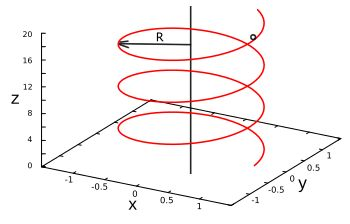
\includegraphics[width=0.6\textwidth]{images/helix.jpg}
    \caption{ Helicoid of radius $R$ }
    \label{image1}
\end{center}
  \end{figure}

  \vspace{5mm}
\section*{Exercise 2 (20 p)}

Watch the link 1 and the scene in the link 2 that happens inside the space station. 
Estimate what is the radius of the space station.
\vspace{3mm}

link 1: \url{https://www.youtube.com/watch?v=0ZoSYsNADtY}

link 2: \url{https://www.youtube.com/watch?v=vG6CjOFlo7A}


\vspace{5mm}
Hint: You must use the second law of Newton and the expressions for circular motion with constant angular acceleration.

\vspace{5mm}
\section*{Exercise 3 (20 p)}
A ball moves in the xy-plane. Its coordinates are given as functions of time by

\begin{equation}
    x(t)=R(\omega t-sin \omega t) \ \ \  y(t)=R(\omega t-cos \omega t)
\end{equation}

where $R$ and $\omega$ are constants.

\begin{itemize}
    \item Choose values for $\omega$ and $R$ and model the motion in 3dsMax.
    \item Look at the curves in curve editor and determine:
    \begin{itemize}
        \item     At which times is
        the ball at rest? What are the coordinates at these times?
        \item Print the curves and the motion path and indicate the answers on the images.
        \item  Compare to the motion in exercise 1, what are the differences?
    \end{itemize}

\end{itemize}





\end{document}


